\chapter{Teoretická část}
\section{Suspendace}
Smyslem suspendace v~mechanicky míchaných nádobách je udržení pevných částic ve vznosu tak, aby došlo ke zintenzivnění transportu hmoty a tepla mezi kapalinou a pevnou fází. Pro dosažení tohoto stavu je třeba systému dodat energii v~podobě mechanické práce. K~vykonání této práce se používají rozmanité typy mechanických míchadel, které jsou voleny podle konkretního charakteru dané úlohy. Dodaná energie poté vede k~vytvoření turbulentního proudění, jenž uvede částice pevné fáze do vznosu a následně je rozptýlí v~kapalině. Nutnou podmínkou pro zajištění tohoto vznosu je potřeba, aby výsledná vertikální složka síly působící na částici byla větší než tíhová síla zmenšená o~sílu vztlakovou. Menší částice jejichž hustota je přibližně rovna hustotě kapalina se po dosažení suspenzních podmínek pohybují společně s~kapalinou. Při nižších koncentracích pevné fáze se toto proudění chová spíše jako jednofázový tok. Naopak rychlost pohybu těžších částic se liší od rychlosti kapalné fáze, jenž musí na pevnou fázi působit větší silou k~zabránění jejímu usazování. Výslednou kvalitu vzniklé suspenze ovlivňuje řada faktorů, kde mezi nejvýznamnější patří fyzikální vlastnosti, jak kapalné, tak pevné fáze, provozní podmínky a geometrie systému a míchadla.

\subsection{Stupně suspendace}
Nároky na homogenitu vsádky se liší dle konkretních provozních požadavků. Jedním z~pojmů, který se používá k~popisu míry homogenizace vsádky v~mechanicky míchaných nádobách je stupeň suspendace. Obecně se rozlišují tři stupně suspendace: částečná, úplná a homogenní (obr. \ref{fig:typsus}). 
  
\begin{figure}[h!]
  \centering
  \subfloat[Částečná]{\label{fig:typ1}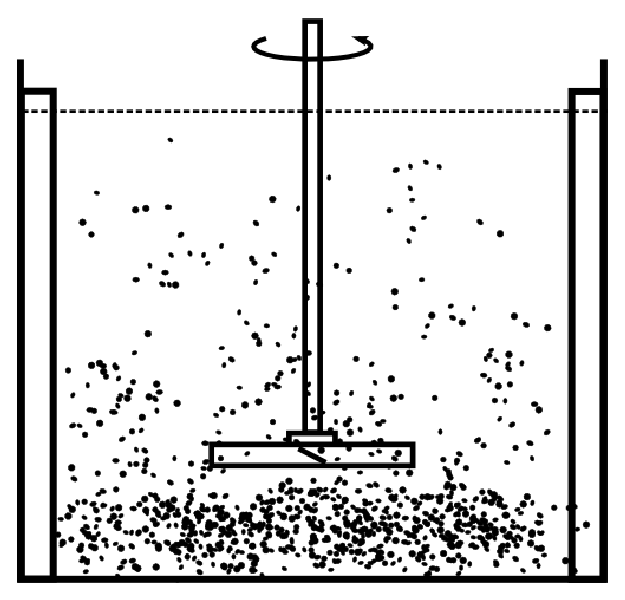
\includegraphics[scale=0.35]{images/typy_suspenzi-1.eps}}
  \qquad
  \subfloat[Úplná]{\label{fig:typ2}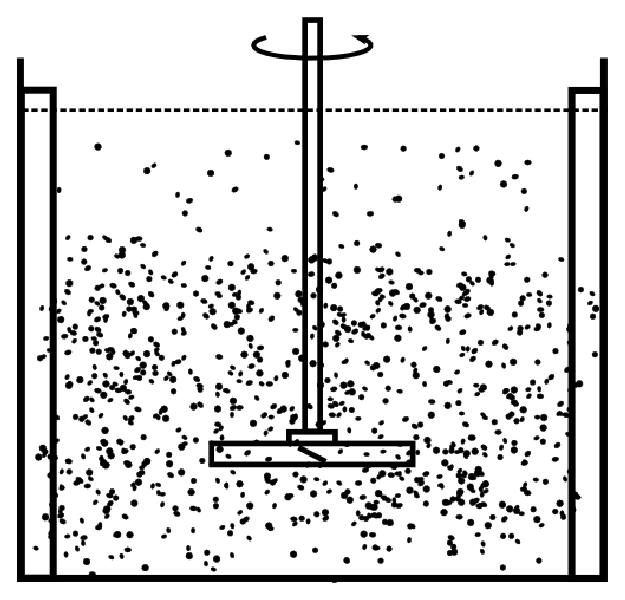
\includegraphics[scale=0.35]{images/typy_suspenzi-2.eps}}
  \qquad
  \subfloat[Homogenní]{\label{fig:typ3}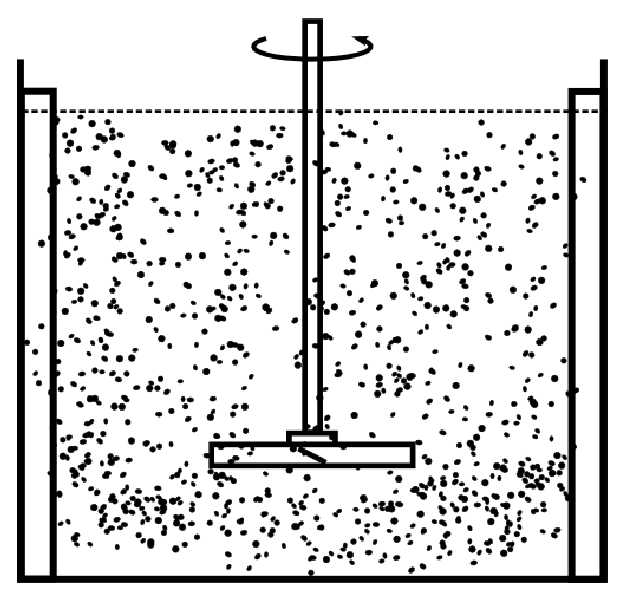
\includegraphics[scale=0.35]{images/typy_suspenzi-3.eps}}
  \caption{Stupně suspendace}
  \label{fig:typsus}
\end{figure}

Při částečné suspendaci lze vizuálně pozorovat pohyb částic pevné fáze pouze v~blízkosti dna nádoby. Toto shlukování má za následek zhoršení přestupu tepla a hmoty, což v~důsledku může snížit rychlost probíhajících chemických reakcí. Z~výše uvedeného vyplývá, že podmínky částečné suspendace jsou postačují pouze při míchaní vysoce rozpustných látek.

Stav úplné suspendace je charakterizován pohybem pevné fáze v~celé nádobě, přičemž žádná částice nezůstává na dně déle než jednu až dvě sekundy. Tato podmínka se někdy označuje jako Zwieteringovo kritérium podle autora, který jako první na základě experimentů navrhl vztah k~výpočtu kritické (minimální) frekvence otáčení míchadla potřebné k~dosažení stavu úplné suspendace. Při tomto stavu je maximální povrch částic vystaven kapalině, což má za následek intenzivní transport hmoty a tepla mezi jednotlivými fázemi.

Posledním stádiem je dosažení stavu homogenní suspendace, při němž částice pevné fáze dosahují prakticky rovnoměrného rozložení v~celém promíchávaném systému. Jakékoliv další zvýšení frekvence míchadla nebo jeho příkonu nemá již prakticky žádný vliv na distribuci pevné fáze. Dosažení stavu homogenní suspendace je často důležité u~procesů, které vyžadují rovnoměrné rozložení částic v~systému. Příkladem takovéhoto procesu může být krystalizace, kde nerovnoměrná koncentrace pevné fáze způsobuje tvorbu míst s~lokálním přesycením, jenž následně negativně ovlivňují kvalitu vzniklých krystalů. Nicméně ve většině případů je postačující dosažení stavu úplné suspendace, který vyžaduje menší množství vykonané práce.

\subsection{Kritická frekvence otáčení míchadla}
Jak již bylo zmíněno v~předcházející kapitole, kritická frekvence otáčení je minimální rychlost otáčení míchadla potřeba k~udržení částic pevné fáze ve vznosu. První kdo navrhl empirickou korelaci k~jejímu výpočtu byl \citet{zwi58}. Jím navržený vztah má tvar:
\begin{equation}
	N_{js} = \left[\frac{g(\rho_{s}-\rho_{l})}{\rho_{l}}\right]^{\num{0.45}}W^{\num{0.13}}d_{p}^{\num{0.2}}D^{\num{-0.85}}\nu^{\num{0.1}}S
	\label{eq:nkrit}
\end{equation} 

\noindent kde $g$ je gravitační zrychlení, $\rho_{s}$ hustota pevné fáze, $\rho_{l}$ hustota kapalné fáze, $W$ relativní hmotnostní zlomek pevné fáze, $d_{p}$ průměr částice pevné fáze, $\nu$ kinematická viskozita a $S$ je bezrozměrná Zwieteringova konstanta, která zohledňuje geometrii systému a míchadla (tab. \ref{tab:S}). Ze vztahu je dobře patrné, že rozdíl hustot jednotlivých fází nejvýznamněji ovlivňuje výslednou kritickou frekvenci otáčení míchadla. Později provedené studie \citep{nie68,bal78,chou97} obecně potvrdily platnost Zwieteringova vztahu. Nicméně \citet{chou97} experimentálně ukázal, že při koncentraci pevné fáze menší než \volproc{2} nebo větší než \volproc{15} se již tato korelace jeví jako nepříliš spolehlivá.

\begin{table}[h!]
\begin{center}
\caption{Zwieteringovy konstanty pro \SI{45}{\degree} PBT}
\label{tab:S}
\begin{tabular}{llr}
\toprule
Šířka lopatky & Světlá výška & Hodnota \\
\midrule

$D/\num{3.5}$ \\
& $T/4$ & \num{4.8} \\
& $T/6$ & \num{4.6} \\
& $T/8$ & \num{3.2} \\
$D/4$ \\
& $T/4$ & \num{4.4} \\
& $T/6$ & \num{4.1} \\
& $T/8$ & \num{3.7} \\

\bottomrule
\end{tabular}
\end{center}
\end{table}

\subsection{Kvalita suspenze (stupeň homogenizace)}
Další užitečnou charakteristikou systému kapalina-pevná fáze je takzvaná kvalita suspenze, což je směrodatná odchylka koncentrace pevné fáze. Často se však dává přednost vyjádření pomocí objemového zlomku pevné fáze. Pro konečný počet $n$ měření lze kvalitu suspenze definovat jako:
\begin{equation}
	\sigma = \sqrt{\frac{1}{n}\sum_{i=1}^{n}\left(\frac{c_{i}}{\bar{c}} - 1\right)^{2}}
	\label{eq:kvasus}
\end{equation}  

\noindent Díky své diskrétní povaze je tato veličina navíc dobře stanovitelná pomocí simulační techniky CFD. S~rostoucí homogenitou systémů číselná hodnota kvality suspenze klesá a v~limitním případě je nulová. Někdy se proto místo kvality suspenze používá pojem stupeň homogenizace, jenž vznikne odečtením kvality suspenze od jedničky.

\citet{boh80} určili na základě experimentů hodnoty kvality suspenze pro jednotlivé stupně suspendace. Jejich výsledky jsou shrnuty v~tab. \ref{tab:kvasus}.

\begin{table}[h!]
\begin{center}
\caption{Rozdělení stupňů suspendace dle kvality suspenze}
\label{tab:kvasus}
\begin{tabular}{cc}
\toprule
Stupeň suspendace & Kvalita suspenze \\
\midrule

Částečná &  $\sigma \geq \num{0.8}$ \\
Úplná & $\num{0.2} < \sigma < \num{0.8}$ \\
Homogenní & $\sigma \leq \num{0.2}$ \\

\bottomrule
\end{tabular}
\end{center}
\end{table}

\subsection{Výška vznosu pevné fáze}
Při míchaní suspenzní se ve vsádce tvoří snadno rozlišitelná oblast ve které se vyskytuje naprostá většina částic pevné fáze. Vzdálenost mezi dnem nádoby a rozhraním této oblasti se někdy také nazývá jako výška suspenzního mraku. 

Experimentálně studovali výšku suspenzního mraku např. autoři \citet{hic97}. Z~jejich měření vyplynulo, že nejvýznamnější vliv na výšku vznosu pevné fáze má poměr průměrů míchadla a nádoby $(D/T)$, poměr světlé výšky a průměru nádoby $(C/T)$ a koncentrace pevné fáze. Dosažení dobré distribuce částic ve vysoké nádobě $(H > T)$ se ukázalo jako poměrně problematické, a proto výzkumníci zdůraznili potřebu použití více míchadel v~takovýchto systémech.

\citet{bit02} odvodili korelaci pro výpočet výšky suspenzního mraku na základě dostupných experimentálních dat, které naměřili \citet{hic97} a \citet{buj99}. Zmíněný vztah byl navržen pro rychloběžná axiální míchadla a má tvar:
\begin{equation}
	C_{H}=\frac{N}{N_{js}}\left[\num{0.84} - \num{1.05}\frac{C}{T} + \num{0.7}\frac{(D/T)^{2}}{1 - (D/T)^{2}}  \right]T
	\label{eq:sushei}
\end{equation}  

\subsection{Doba homogenizace}
Doba homogenizace $t_{mix}$ je definována jako čas potřebný k tomu, aby se hodnota normalizované koncentrace stopovací látky $c(t)^{*}$ pohybovala v předem zvoleném rozmezí. Nejčastěji se volí přípustná hodnota fluktuace \SI{\pm 5}{\percent}, tedy $c(t)^{*} \in \left<\num{0.95};\num{1.05}\right>$. 

Výše zmíněná normalizovaná kocentrace je určena vztahem:
\begin{equation}
	c(t)^{*} = \frac{c(t) - c_{0}}{c_{\infty} - c_{0}}
	\label{eq:bezkon}
\end{equation}

\noindent přičemž $c(t)$ je koncentrace stopovací látky v čase $t$, $c_{\infty}$ je koncentrace ve vsádce po dokonalém rozmíchání a $c_{0}$ představuje počáteční koncentraci v systému.  

Hodnota doby homogenizace také velmi záleží na místě měření zmíněné koncentrace. Například \citet{buj99} měřili dobu homogenizace pro systém kapalina-pevná fáze v mechanicky míchané nádobě. Z výsledků vyplynulo, že nad suspenzním mrakem je doba homogenizace přibližně dvacetkrát delší než v oblasti, která je bohatá na přítomnost částic pevné fáze.

%\newpage 
\section{Počítačová dynamika tekutin (CFD)}
Následující kapitola obsahuje stručný přehled základních rovnic a matematických modelů, které jsou uplatněny při simulaci pomocí techniky CFD. Hlavní důraz je kladen na problematiku isotermního vícefázového proudění kapalina-pevná fáze v mechanicky míchaných nádobách.

\subsection{Úvod do CFD}
Počítačová dynamika tekutin (angl. computational fluid dynamics -- CFD) je jedno z odvětví hydromechaniky, jenž využívá numerické metody a algoritmy k řešení problémů zahrnující proudění tekutin, transport hmoty a tepla, chemické reakce a celou řadu dalších fyzikálně-chemických jevů. Na počátku každé CFD simulace je třeba nejprve vytvořit model zkoumaného systémů na který jsou následně aplikovány matematické postupy tak, aby byly ze zadaných okrajových a počátečních podmínek získány vybrané údaje o dějích probíhajících v celé zkoumané doméně při respektování fyzikálních zákonů. Tyto zákony jsou nejčastěji formulovány v podobě parciálních diferenciálních rovnic. 

S prudkým nárůstem výkonu výpočetní techniky se metoda CFD stala přístupnější širšímu množství uživatelů. Mezi její hlavní výhody patří schopnost studovat systém za podmínek, kdy experimentální měření jsou těžko proveditelná, či přímo nemožná. Díky tomu je možné např. dosáhnout znatelného snížení finančních a časových nákladů ve vývojové fází nového výrobku. Nicméně je třeba dodat, že každý simulační výpočet je silně závislý na dodaných počátečních a okrajových podmínkách, a proto CFD nikdy nemůže úplně nahradit experimentální měření.

Celou CFD simulaci lze rozdělit do třech hlavních kroků: tvorba geometrie a výpočetní sítě, vlastní výpočet a analýza výsledků

\subsubsection{Tvorba geometrie a výpočetní sítě (preprocessing)}
V první fází je vytvořena geometrie zkoumaného systému, která je následně rozdělena na konečný počet kontrolních objemů (buněk). Vzniklá výpočetní síť může obsahovat buňky různých typů. Dvojrozměrná doména se nejčastěji dělí na trojúhelníky nebo obdélníky. V trojrozměrném případě se nejčastěji využívají jehlany, hranoly, kvádry či další mnohostěny. V současnosti se již dává přednost nestrukturovaným sítím před strukturovanýma. Pro strukturovanou síť platí, že každá stěna buňky přiléhá pouze k jedné stěně sousedního kontrolního objemu. Jejich hlavní nevýhodou je obtížná tvorba složitějších tvarů a nemožnost libovolného zahušťování.

\subsubsection{Vlastní výpočet}
K provedení vlastního simulačního výpočtu dnes existuje celá řada jak komerčních, tak bezplatných CFD řešičů. Příkladem komerčních produktů může být např. ANSYS Fluent, ANSYS CFX,  ANSYS Polyflow nebo STAR-CCM+. Mezi nejznámější bezplatné CFD řešiče patří OpenFOAM či Code Saturne. Interně tyto softwary využívají jednu z následujích numerických metod k řešení parciálních diferenciálních rovnic:

\begin{itemize}[itemsep=0pt,parsep=0pt,partopsep=0pt,topsep=0pt]
  \item \textbf{Metoda konečných diferencí (FDM)}
  
  Tato metoda, někdy též označována jako metoda sítí, patří mezi nejstarší techniky k řešení parciálních diferenciálních rovnic. Její podstatou je náhrada derivací pomocí diferenčních náhrad, což má za následek diskretizaci daného problému na konečný počet uzlů. Ve výsledku se tedy řeší soustava lineárních algebraických rovnic. Mezi jednu z hlavních nevýhod této metody je její obtížná formulace pro nestrukturované sítě. 
  \item \textbf{Metoda konečných objemů (FVM)}
  
  Hlavním znakem metody konečných objemů je fakt, že řeší rovnice modelu v integrální formě pro konečný počet kontrolních objemů. Díky tomu je zaručeno splnění zákonů zachování dané veličiny pro každou výpočetní buňku. Následná diskretizace výše zmíněných integrálních rovnic převádí opět vede na řešení řídké soustavy lineárních algebraických rovnic. Drtivá většina dnešních CFD rešičů využívá právě tuto numerickou metodu. 
  
  \item \textbf{Metoda konečných prvků (FEM)}
  
  Podstatou metody konečných prvků je hledání řešení daných parciálních diferenciálních rovnic v podobě po částech definovaných funkcí na předem zvoleném počtu buněk. Ve výsledku se tedy hledají váhové koeficienty pro tyto bázové funkce tak, aby získané řešení minimalizovalo chybu aproximace. Metoda konečných prvků je zvláště využívána v oblasti pevnostní analýzy nebo při simulaci proudění vysoce nenewtonovských tekutin.  
\end{itemize}

\subsubsection{Analýza výsledků (postprocessing)}
Posledním krokem každé CFD je zpracování a analýza získaných simulačních výsledků. K tomuto účelu bylo vytvořena řada softwarových nástrojů mezi které patří např. Ansys CFD-Post, Tecplot 360 nebo ParaView. Hlavní úkoly těchto programů činí:

\begin{itemize}[itemsep=0pt,parsep=0pt,partopsep=0pt,topsep=0pt]
  \item výpočet dodatečných veličin
  \item tvorba řezů doménou
  \item zobrazení vektorových polí
  \item tvorba konturových grafů
  \item vyobrazení ploch o konstantní hodnotě veličiny
  \item porovnání několika simulací
\end{itemize}

\subsection{Rovnice kontinuity}

Základní vztahem pro popis tekutiny je rovnice kontinuity, jenž vyjadřuje zákon zachování hmoty. Pro jednofázový systém obsahující stlačitelnou tekutinu má tato rovnice tvar:
\begin{equation}
	\frac{\partial \rho}{\partial t} + \nabla \cdot (\rho\vec{v}) = 0
	\label{eq:conti1}
\end{equation}
přičemž $\rho$ značí hustotu tekutiny, $t$ čas a $\vec{v}$ je vektor rychlosti. První člen v rov. \ref{eq:conti1} reprezentuje změnu hustoty v čase (akumulaci) a druhý člen představuje změnu hmotnosti objemového elementu v důsledku konvekce. Pokud lze tekutinu považovat za nestlačitelnou, tak hustota kontinua je konstantní a výše zmíněný vztah se zjednoduší na rov. \ref{eq:conti1simp}.
\begin{equation}
	\nabla \cdot \vec{v} = 0
	\label{eq:conti1simp}
\end{equation}  

Pro vícefázový systém je třeba zapsat rovnici kontinuity pro každou fázi zvlášť, přičemž je třeba obecně uvažovat přenos hmoty mezi jednotlivými fázemi. Rovnice kontinuity pro $i$-tou fázi lze zapsat jako:
\begin{equation}
	\frac{\partial}{\partial t} (\alpha_{i}\rho_{i}) +  \nabla \cdot (\alpha_{i}\rho_{i}\vec{v}_{i}) = \sum_{\substack{ i \neq j \\ j=1}}^{n}\Gamma_{ij}
	\label{eq:conti2}
\end{equation} 
kde člen $\Gamma_{ij}$ představuje hmotnostní tok mezi $i$-tou a $j$-tou fází vztažený na objemový element a $\alpha_{i}$ značí objemový zlomek dané fáze. Objemové zlomky všech fází navíc musí splňovat algebraickou rovnici \ref{eq:volfrac}.
\begin{equation}
	\sum_{i=1}^n \alpha_{i} = 1
	\label{eq:volfrac}
\end{equation} 

\subsection{Bilance hybnosti}
